\chapter{動作実験}

\section{esaで記事を書く}
  今回はこの二つを投稿したとします。

  \begin{figure}[H]
    \centering
    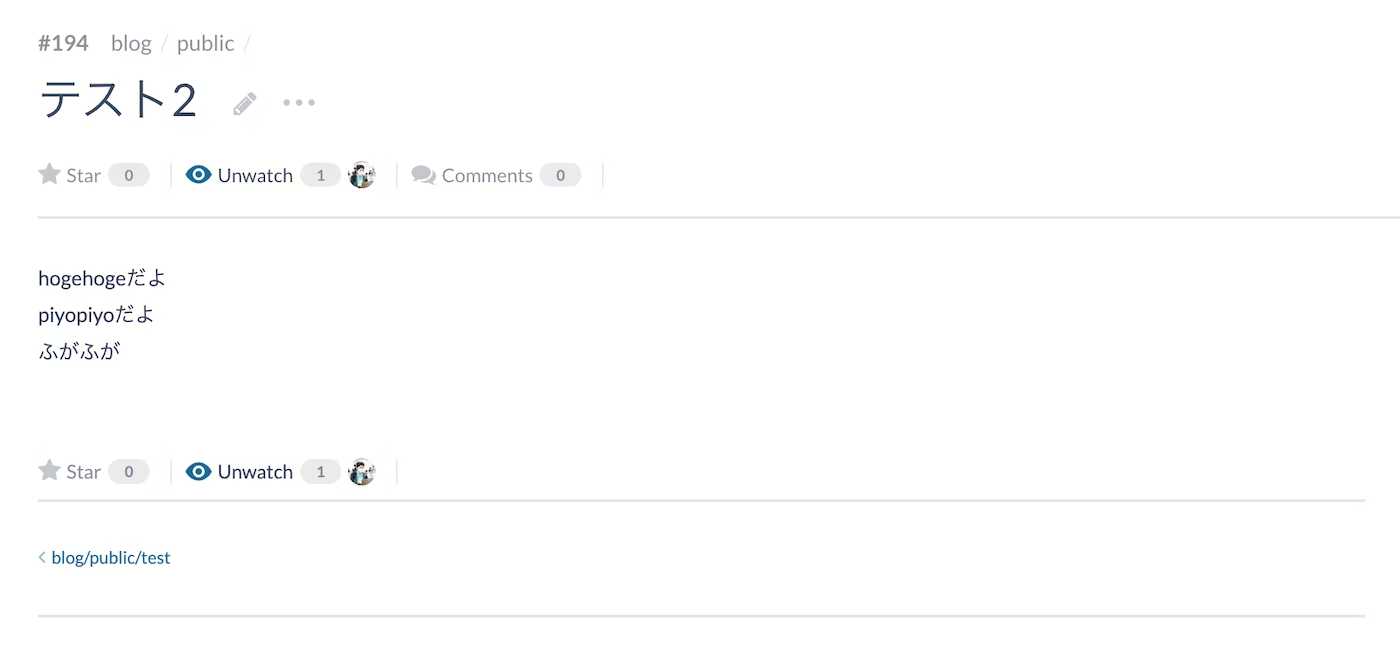
\includegraphics[width=8cm]{./image/02-chap9/esa-post-1.png}
    \caption{esaに投稿した記事1}
    \label{chap9-esa-post-1-image}
  \end{figure}

  \begin{figure}[H]
    \centering
    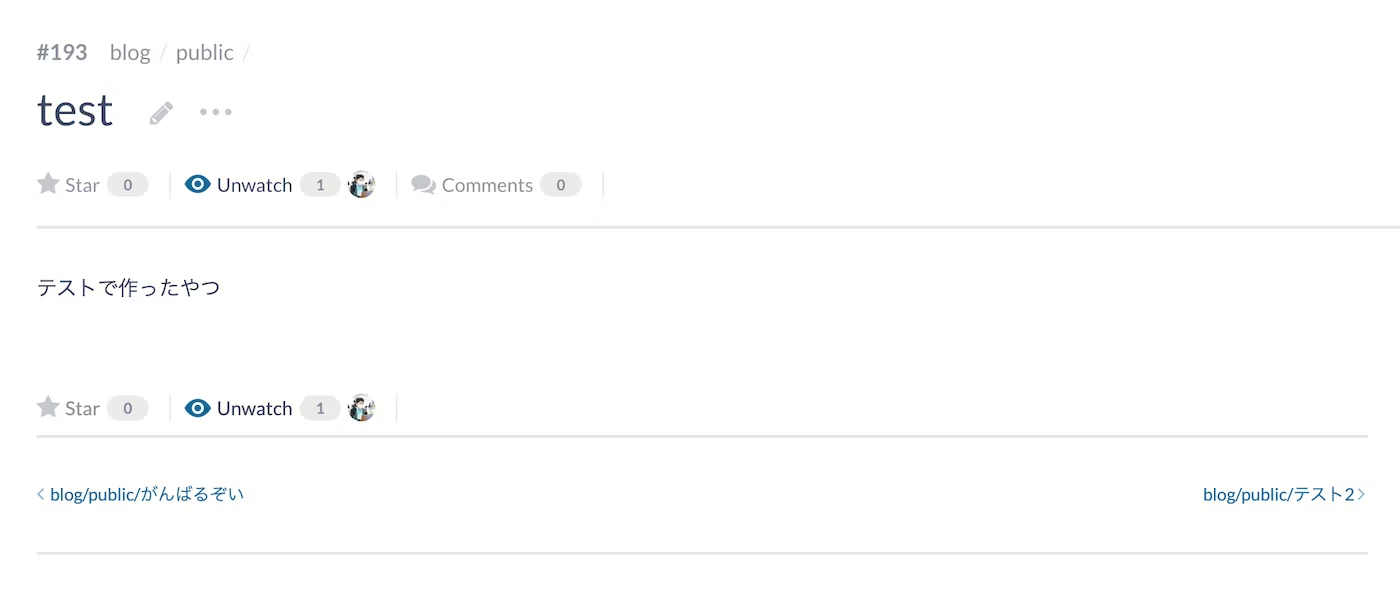
\includegraphics[width=8cm]{./image/02-chap9/esa-post-2.png}
    \caption{esaに投稿した記事2}
    \label{chap9-esa-post-2-image}
  \end{figure}

\section{GitHubの状態}

  しばらくすると、esaのWebhooksが走って、mdを保存してくれます。

  \begin{figure}[H]
    \centering
    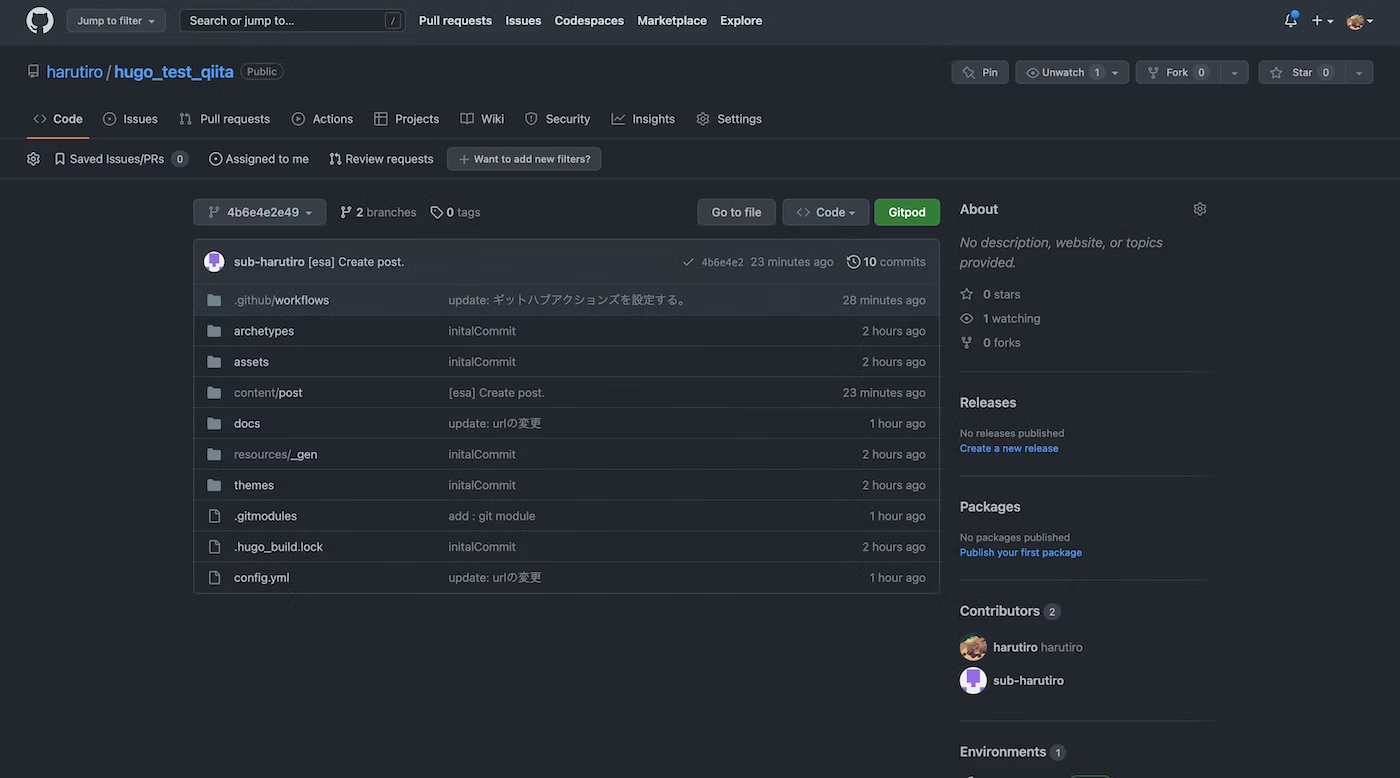
\includegraphics[width=8cm]{./image/02-chap9/git-repo.png}
    \caption{gitのリポジトリの状態}
    \label{chap9-git-repo-image}
  \end{figure}

\section{GitHub Actionsの状態}
  あたらしくPushされると、GitHub Actionsが走って、web$\_$publicのブランチに静的ファイルが生成されます。

  \begin{figure}[H]
    \centering
    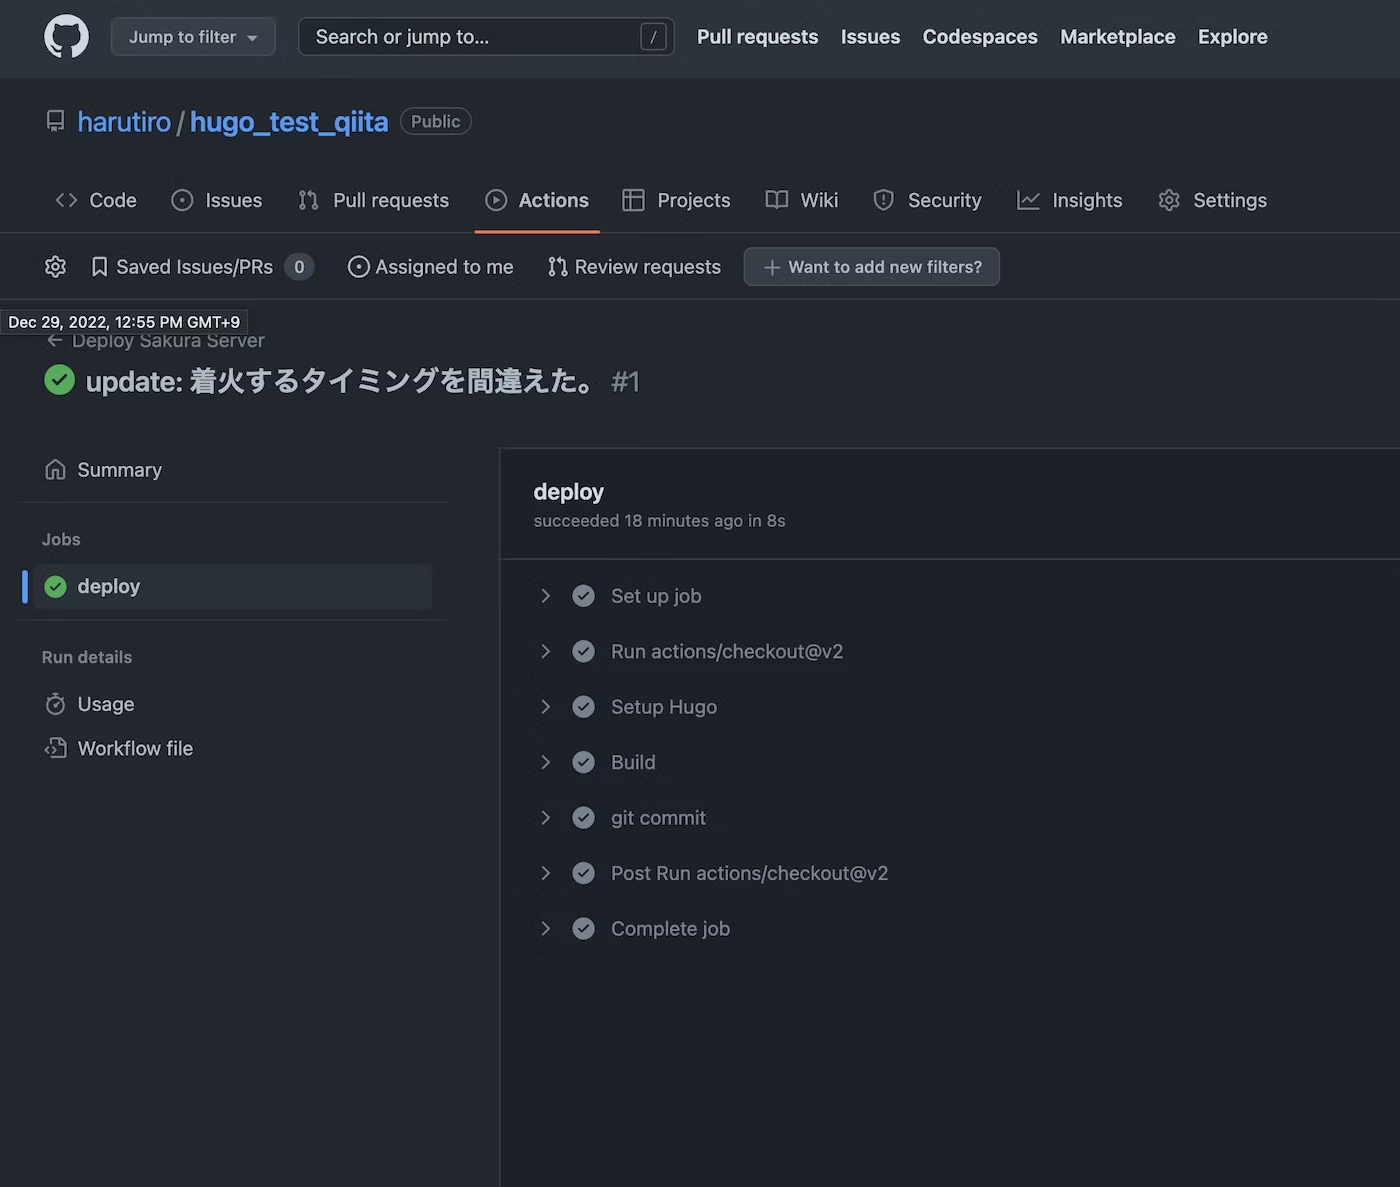
\includegraphics[width=8cm]{./image/02-chap9/git-action1.png}
    \caption{GitHub Actionsの状態}
    \label{chap9-git-action1-image}
  \end{figure}

  \begin{figure}[H]
    \centering
    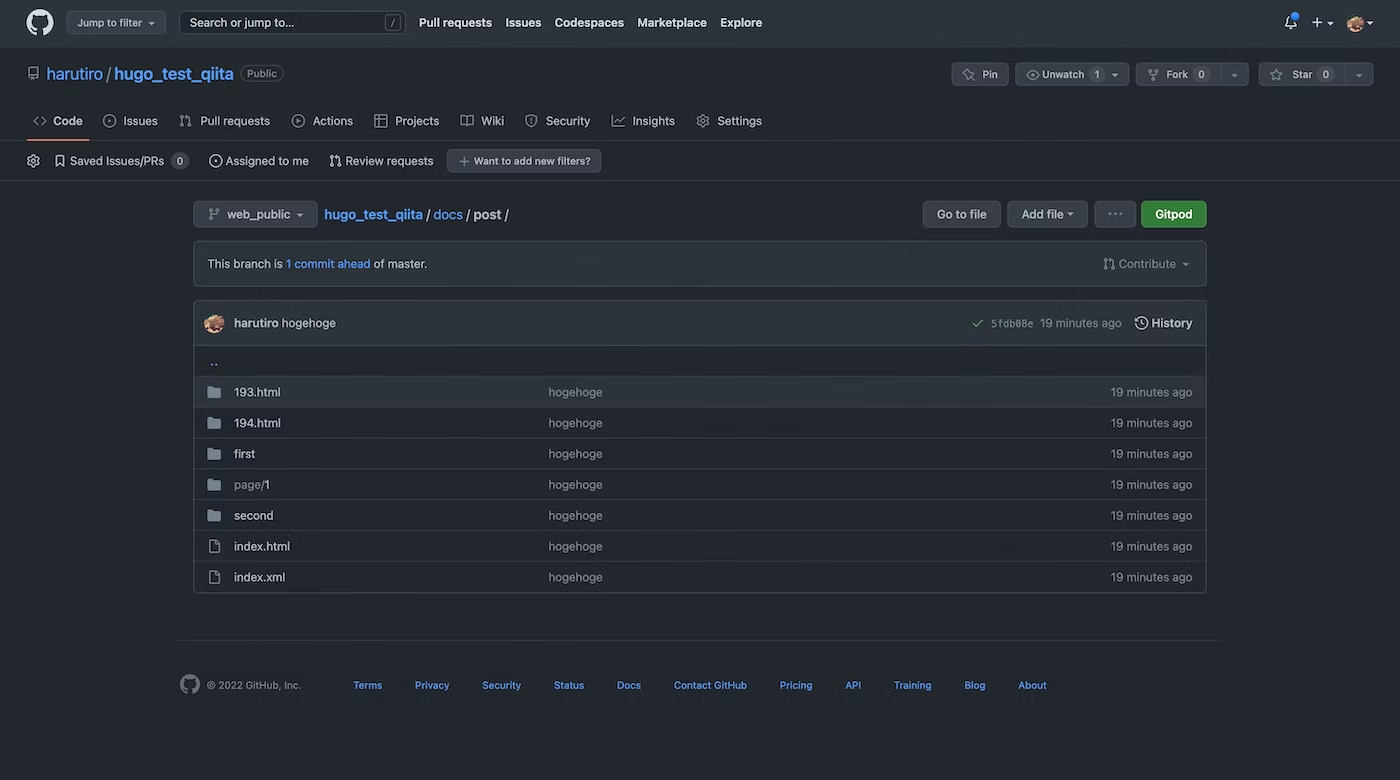
\includegraphics[width=8cm]{./image/02-chap9/git-action2.png}
    \caption{GitHub Actionsの状態 hugoの生成をしている状態}
    \label{chap9-git-action2-image}
  \end{figure}

\section{GitHub Pagesの状態}
  web$\_$publicにpushされるとGitHub Pagesが走って、自動的にデプロイされます。

  \begin{figure}[H]
    \centering
    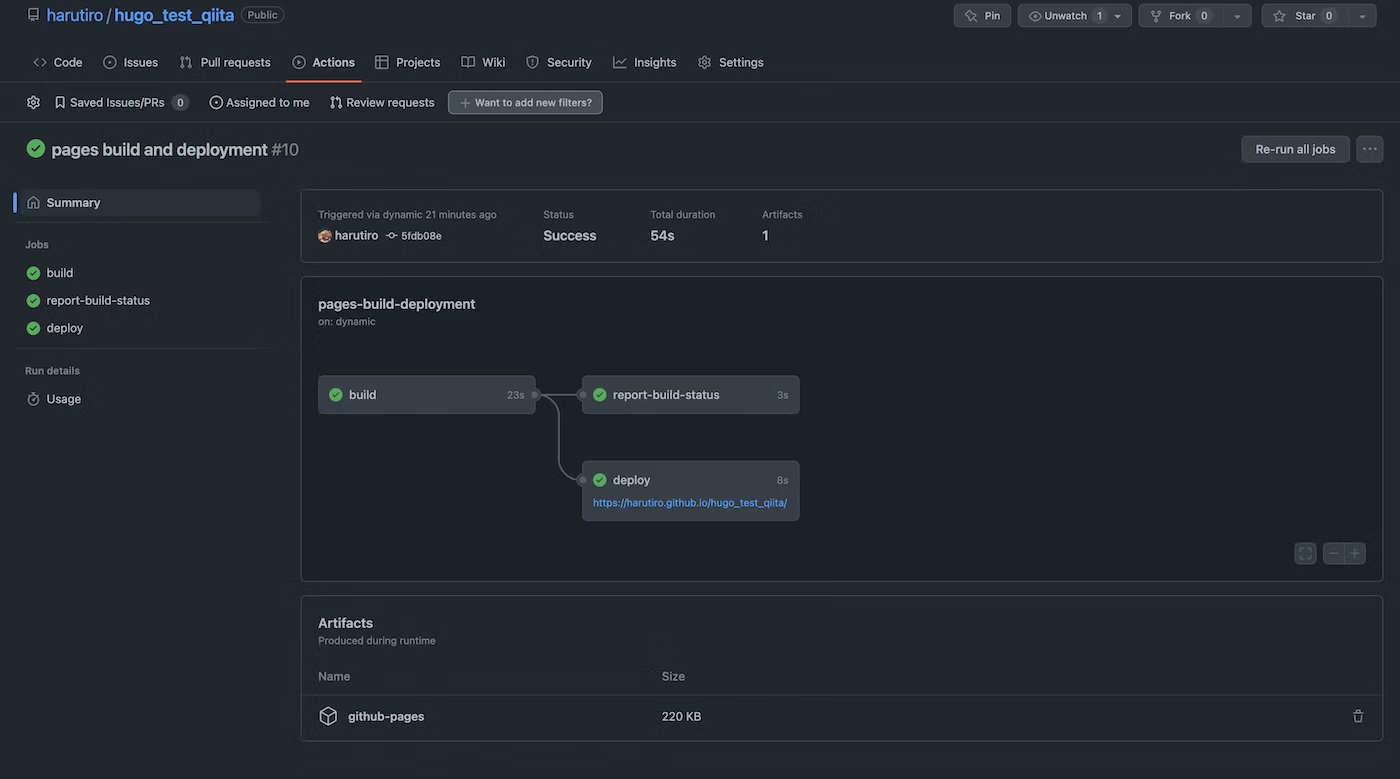
\includegraphics[width=8cm]{./image/02-chap9/git-pases.png}
    \caption{GitHub Pagesの状態}
    \label{chap9-git-pases-image}
  \end{figure}

\section{webページの状態}
  自動で更新がされていることが確認できました。

  \begin{figure}[H]
    \centering
    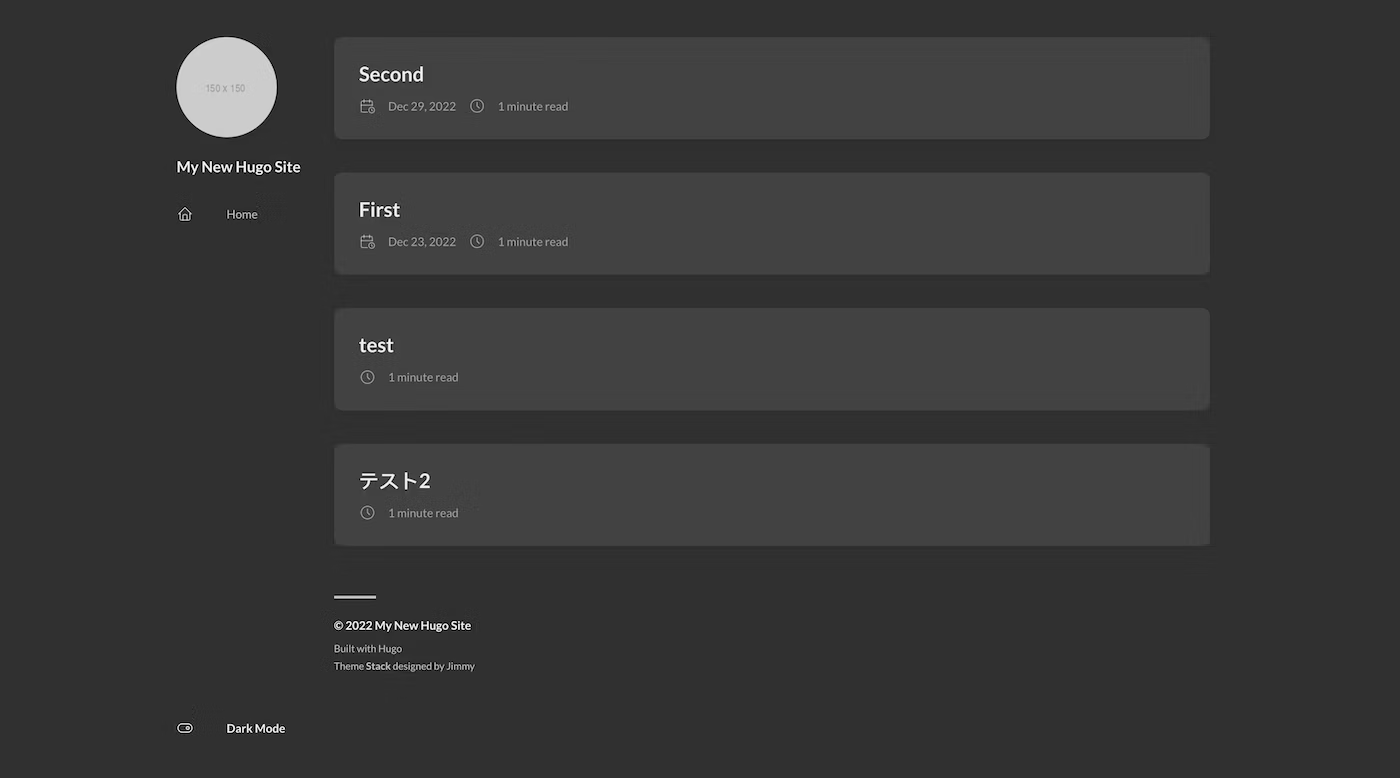
\includegraphics[width=8cm]{./image/02-chap9/hugo1.png}
    \caption{webページの状態}
    \label{chap9-hugo1-image}
  \end{figure}

  \begin{figure}[H]
    \centering
    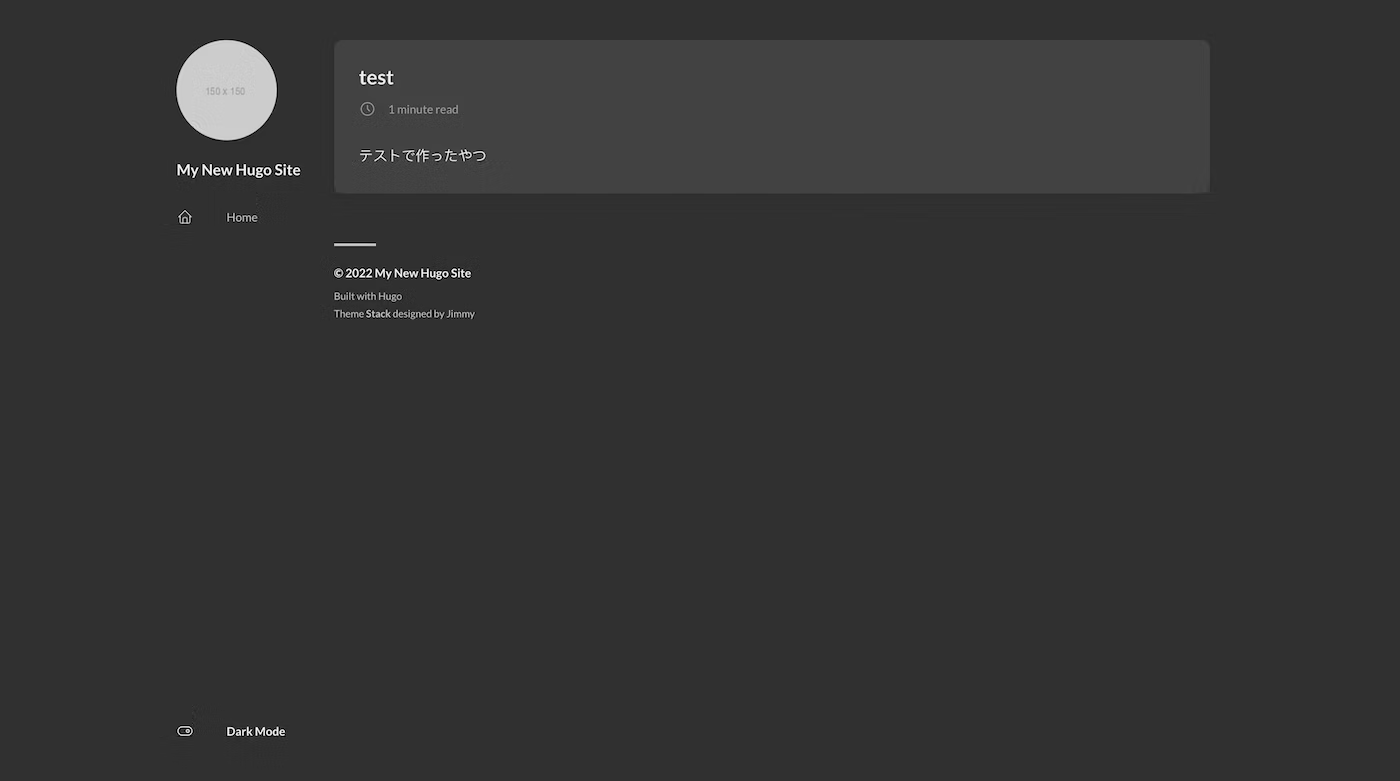
\includegraphics[width=8cm]{./image/02-chap9/hugo2.png}
    \caption{webページの状態 記事1}
    \label{chap9-hugo2-image}
  \end{figure}

  \begin{figure}[H]
    \centering
    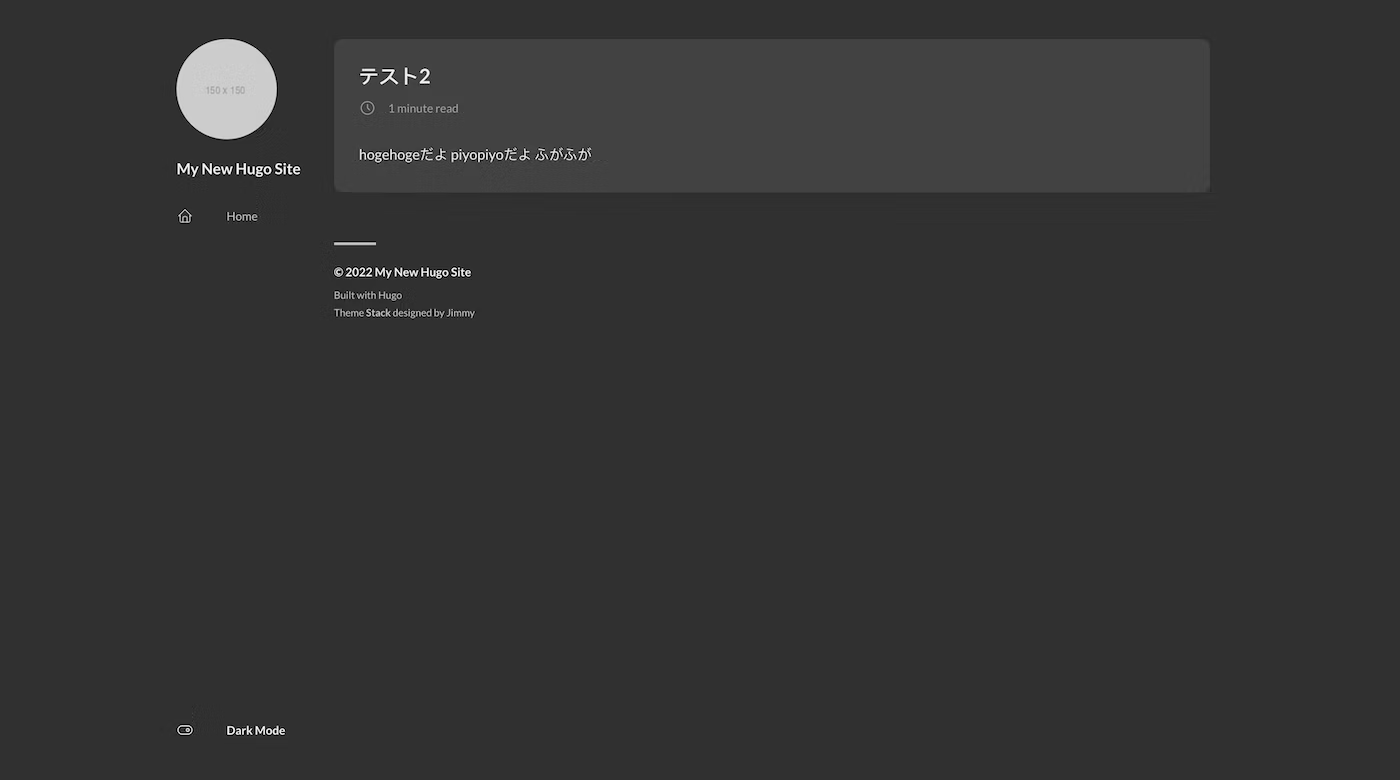
\includegraphics[width=8cm]{./image/02-chap9/hugo3.png}
    \caption{webページの状態 記事2}
    \label{chap9-hugo3-image}
  \end{figure}